\documentclass[a4paper,oneside,12pt]{amsart}

%\usepackage[spanish, activeacute]{babel}
\usepackage[utf8]{inputenc}
%\usepackage[latin1]{inputenc}
\usepackage{latexsym}
\usepackage{multicol}
\usepackage{enumerate}
\usepackage{enumitem}
\usepackage[heightrounded]{geometry}
\geometry{top=2cm,bottom=2cm,left=2cm,right=2cm}
\usepackage{graphicx}
\usepackage{tikz}
\usetikzlibrary{graphs, graphs.standard}
\usepackage{amssymb}
\usepackage{tikz-network}

\DeclareMathOperator{\cond}{cond}
\DeclareMathOperator{\Id}{Id}
\DeclareMathOperator{\re}{Re}
%\DeclareMathOperator{\im}{Im}
\newcommand{\I}{\mathbb{I}}
\newcommand{\R}{\mathbb{R}}
\newcommand{\Q}{\mathbb{Q}}
\newcommand{\C}{\mathbb{C}}
\newcommand{\Z}{\mathbb{Z}}
\newcommand{\N}{\mathbb{N}}
\DeclareMathOperator{\im}{Im}

\newcommand{\nombremateria}
{Investigaci\'on Operativa}
\newcommand{\nombrecuatrimestre}
    {Segundo cuatrimestre de 2025}
\newcommand{\numeroparcial}
    { Recuperatorio del Tercer Parcial }
\newcommand{\fecha}
    {23 de Diciembre de 2025}
\newcommand{\numerotema}
    {\bf 1}

%\oddsidemargin -1cm \evensidemargin -1cm \textwidth 17.5cm
%topmargin 1.2cm \textheight 25cm
%\setlength{\textheight}{25cm}

\def \ds{\displaystyle}
\theoremstyle{definition}
\newtheorem{quest}{Ejercicio}
\thispagestyle{empty}

\begin{document}

\hfill \hfill
\begin{tabular}[c]{|c|c|c|c|}
\hline 
1 & 2 & 3 & Calificaci\'on \\ \hline \hline
\hspace{1.2 cm} & \hspace{1.2 cm} & \hspace{1.2 cm} &\hspace{1.5 cm} \\
\hspace{1.2 cm} & \hspace{1.2 cm} & \hspace{1.2 cm} &\hspace{1.5 cm} \\ \hline

\end{tabular}

\vspace{-1cm}

\noindent Nombre y apellido:

\vspace{0.2cm}

\noindent Número de libreta:

\noindent \hrulefill 

\smallskip
\renewcommand{\baselinestretch}{1.1}

\begin{center}
	\large \textbf{\nombremateria} 
	
	\numeroparcial -- \fecha
\end{center}

\begin{center}
\textbf{Entregue todos los ejercicios en hojas separadas.}
\end{center}

\vspace{.6cm}
\renewcommand{\theenumi}{\textbf{\arabic{enumi}}}

%%% EMPIEZA EL EJERCICIO 1 %%%

\begin{quest}\verb|[3.5 pts.]|
Demostrar las siguientes afirmaciones. Cada ítem se puede demostrar individualmente, no es necesario utilizar el
resultado de los demás.
%\noindent
\begin{enumerate}[label=\alph*)]
    \item \verb|[0.75 pts.]| Demostrar que todo grafo tiene un vértice $v$ tal que $d(v) \leq \frac{2m}{n}$ y un
    vértice $w$ tal que
    $d(w) \geq \frac{2m}{n}$ donde $m$ es la cantidad de aristas y $n$ la cantidad de vértices del grafo.
    \item \verb|[1 pt.]| Sea $T$ un árbol generador mínimo de un grafo pesado conexo
    $\mathcal{G}=(\mathbb{V}, \mathbb{E})$ y sea
    $\mathbb{V}'\subset \mathbb{V}$. Sea $T'$ el subgrafo de $T$ inducido por $\mathbb{V}'$ y sea $\mathcal{G}'$
    el subgrafo de $\mathcal{G}$ inducido por $\mathbb{V}'$. Demostrar que si $T'$ es conexo, entonces $T'$
    es un árbol generador mínimo de $\mathcal{G}'$.
    \item \verb|[1 pt.]| Sean $\mathcal{G}_1=(\mathbb{V}_1, \mathbb{E}_1)$ y $\mathcal{G}_2(\mathbb{V}_2, \mathbb{E}_2)$
    grafos conexos sin vértices en común. Sean $u\in \mathbb{V}_1$, $v\in \mathbb{V}_2$,
    $\mathcal{G}_3=(\mathbb{V}_1\cup \mathbb{V}_2, \mathbb{E}_1\cup \mathbb{E}_2\cup \{e\})$ siendo $e$
    la arista que conecta a $u$ y a $v$. Mostrar que si existe un circuito euleriano en $\mathcal{G}_1$
    y existe un circuito euleriano en $\mathcal{G}_2$, entonces $\mathcal{G}_3$
    tiene camino euleriano y no tiene circuito euleriano.
    \item \verb|[0.75 pts.]| Sea $\mathcal{G}$ un grafo conexo planar, mostrar que $\delta(\mathcal{G})\leq 5$
    (es decir, existe al menos un vértice con grado menor o igual a $5$).
\end{enumerate}
\end{quest}

%%% TERMINA EL EJERCICIO 1 %%%

%%% EMPIEZA EL EJERCICIO 2 %%%


\begin{quest}\verb|[3.5 pts.]|
Sea $G$ el siguiente grafo:

    \begin{center}
        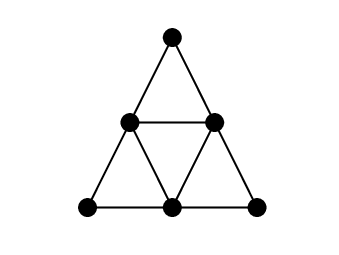
\includegraphics[]{../2021/Imagenes/The-Hajos-Graph.png}
    \end{center}

    \begin{enumerate}[label=\alph*)]
        \item \verb|[0.75 pts.]| Calcular el polinomio cromático de $G$. Justificar.%\\
%        \textbf{Sugerencia:} recordar que el polinomio cromático de $C_n$ es $P(k)=(k-1)^n + (-1)^n(k-1)$
        \item \verb|[0.5 pts.]| Calcular el número cromático de $G$. Justificar.
        \item \verb|[0.75 pts.]| Calcular el índice cromático de $G$. Justificar.
        \item \verb|[0.5 pts.]| Decimos que un grafo es circular si se lo puede representar mediante cuerdas en un
        círculo, de manera tal que cada cuerda representa un vértice y dos cuerdas se intersecan si y solo si los
        correspondientes vértices son adyacentes en $G$. Por ejemplo:
             \begin{center}
            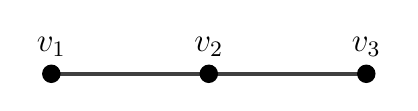
\begin{tikzpicture}
                \SetVertexStyle[FillColor=black, MinSize=0.7]
                \Vertex[label=$v_1$, position=above, fontsize=\large, x=0, y=0]{s1}
                \Vertex[label=$v_2$, position=above, fontsize=\large, x=2, y=0]{s2}
                \Vertex[label=$v_3$, position=above, fontsize=\large, x=4, y=0]{s3}
                \Edge(s1)(s2)
                \Edge(s2)(s3)
            \end{tikzpicture} \hspace{2cm}
        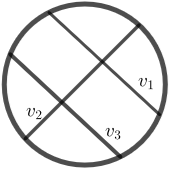
\includegraphics[scale=0.55]{grafo_circular_2}
        \end{center}
        ¿Es $G$ un grafo circular? Justificar.
        \item \verb|[0.5 pts.]| Un grafo se dice ``arco-circular'' si es el grafo intersección de arcos abiertos
        alrededor de un círculo, es
        decir, si se pueden representar sus vértices a través de dichos arcos de modo de que cada arco está
        asociado a un vértice y dos vertices son adyacentes si y solo si los arcos se intersectan. Por ejemplo:
        \begin{center}
            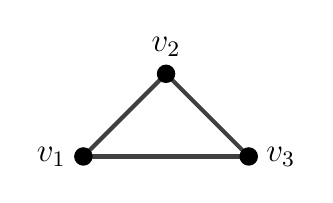
\begin{tikzpicture}[scale=0.7]
                \SetVertexStyle[FillColor=black, MinSize=0.7]
                \Vertex[label=$v_1$, position=left, fontsize=\large, x=0, y=0]{v1}
                \Vertex[label=$v_2$, position=above, fontsize=\large, x=1.5, y=1.5]{v2}
                \Vertex[label=$v_3$, position=right, fontsize=\large, x=3, y=0]{v3}
%                \Vertex[label=$v_4$, position=below, fontsize=\large, x=1.5, y=-1.5]{v4}
                \Edge(v1)(v2)
                \Edge(v2)(v3)
                \Edge(v3)(v1)
%                \Edge(v4)(v1)
            \end{tikzpicture}\hspace{2cm}
%        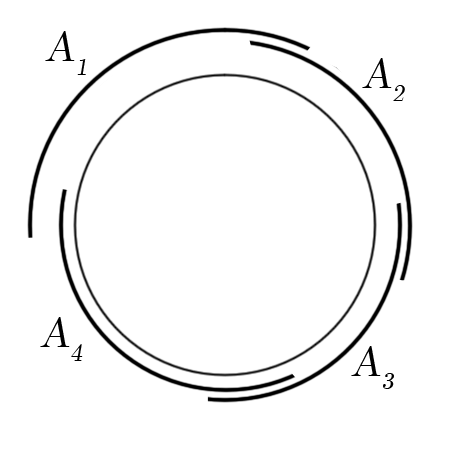
\includegraphics[scale=1]{../2021/Imagenes/arc.png}
            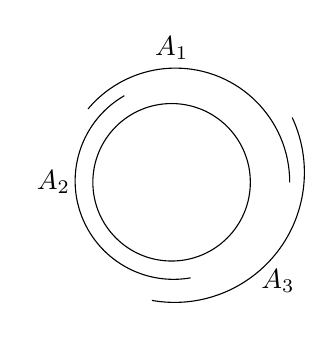
\begin{tikzpicture}
                \draw (0,0) circle(1);
                \draw (1.5,0) arc (0:140:1.45);
                \draw (-0.6,1.1) arc (120:280:1.25);
                \draw (-0.25,-1.5) arc (260:385:1.65);

                \node at (-1.5,0) (A) {$A_2$};
                \node at (0,1.7) (B) {$A_1$};
                \node at (1.35,-1.25) (B) {$A_3$};
            \end{tikzpicture}
        \end{center}
        ¿Es $G$ un grafo arco-circular? Justificar.
        \item \verb|[0.5 pts.]| Un grafo $G$ es de \textit{comparabilidad}
        si existe una orientación transitiva de sus aristas. Es decir, si se pueden orientar todas las aristas del grafo
        de modo de que si existe el arco $u\rightarrow v$ y existe el arco $v\rightarrow w$, entonces debe existir el arco $u\rightarrow w$.

        Por ejemplo, $P_3$:

        \begin{center}
            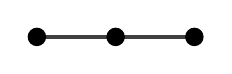
\begin{tikzpicture}
                \SetVertexStyle[FillColor=black, MinSize=0.7]
                \Vertex[x=0, y=0]{n1}
                \Vertex[x=1, y=0]{n2}
                \Vertex[x=2, y=0]{n3}

                \Edge[](n1)(n2)
                \Edge[](n2)(n3)
            \end{tikzpicture}
        \end{center}

        es de comparabilidad, dado que puede orientarse en cualquiera de estas dos formas:

        \begin{center}
            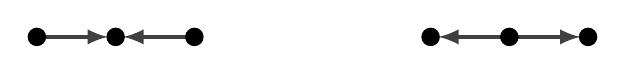
\begin{tikzpicture}
                \SetVertexStyle[FillColor=black, MinSize=0.7]
                \Vertex[x=0, y=0]{n1}
                \Vertex[x=1, y=0]{n2}
                \Vertex[x=2, y=0]{n3}

                \Edge[Direct](n1)(n2)
                \Edge[Direct](n3)(n2)

                \Vertex[x=5, y=0]{n4}
                \Vertex[x=6, y=0]{n5}
                \Vertex[x=7, y=0]{n6}

                \Edge[Direct](n5)(n4)
                \Edge[Direct](n5)(n6)
            \end{tikzpicture}
        \end{center}
        ¿Es $G$ un grafo de comparabilidad? Justificar.
    \end{enumerate}
\end{quest}

%%% TERMINA EL EJERCICIO 2 %%%

%%% EMPIEZA EL EJERCICIO 3 %%%

\begin{quest}
    \verb|[3 pts.]|
    El proceso de manufactura de una joya comienza con un pedazo de plata en bruto. La plata se tiene que
    \textit{tallar}, \textit{pulir}, \textit{agujerear} y \textit{marcar} de manera conveniente:
    \begin{itemize}
        \item Hay que tallarla antes que agujerearla.
        \item Hay que pulirla antes que marcarla.
    \end{itemize}
    Además, cada acción demora una cierta cantidad de tiempo.
    \begin{itemize}
        \item El tallado demora 1 unidad de tiempo.
        \item El pulido demora 1 unidad de tiempo.
        \item El marcado requiere de 2 unidades de tiempo si la pieza no está tallada y 4 unidades de
        tiempo si la pieza está tallada.
        \item Agujerearla requiere de 3 unidades de tiempo si la pieza no está pulida. Si la pieza está pulida, pero
        no marcada, entonces agujerearla requiere de 5 unidades de tiempo. Por otro lado, si la pieza
        está pulida y también marcada, se requieren 7 unidades de tiempo para agujerearla.
    \end{itemize}

    Exhibir el grafo con el cual modelarías el proceso de manufactura de la joya y justificar cuál de los algoritmos
    vistos en clase podría utilizarse para realizar las acciones necesarias en el menor tiempo posible.
\end{quest}

%%% TERMINA EL EJERCICIO 3 %%%

%%% TERMINA EL PARCIAL %%%



\end{document}

